\documentclass[../main.tex]{subfiles}


\begin{document}

\chapter{MATLAB Fundamentals}

\label{cha:cha3}


\begin{center}
\Large{\textbf{CHAPTER OBJECTIVES}}
\end{center}

\normalsize{The primary objective of this chapter is to provide an introduction and overview of
how MATLAB’s calculator mode is used to implement interactive computations.
Specific objectives and topics covered are}

\begin{itemize}



	\item Learning how real and complex numbers are assigned to variables
	\item  Learning how vectors and matrices are assigned values using simple assignment,
the colon operator, and the linspace and logspace functions.
\item  Understanding the priority rules for constructing mathematical expressions.
\item  Gaining a general understanding of built-in functions and how you can learn more
about them with MATLAB’s Help facilities.
\item  Learning how to use vectors to create a simple line plot based on an equation.
\end{itemize}
\Large{YOU'VE GOT A PROBLEM}
\normalsize

n Chap. 1, we used a force balance to determine the terminal velocity of a free-falling
object like a bungee jumper.

$$v_t=\sqrt{\dfrac{gm}{c_d}}  $$

where $v_t =$ terminal velocity (m/s), $g =$ gravitational acceleration ($m/s2$
), $m =$ mass (kg),
and $c_d =$ a drag coefficient (kg/m). Aside from predicting the terminal velocity, this equation can also be rearranged to compute the drag coefficient
 
\begin{equation}
	\tag{2.1}
	c_d = \dfrac{mg}{v^2_t}
\end{equation} 



	\begin{table}[H]
		\centering
		\caption{Data for the mass and associated terminal velocities of a number of jumpers.}
		\begin{tabular}{cccccccc}
			\hline
			$m, kg$ 	&83.6 &60.2 &72.1 &91.1 &92.9 &65.3 &80.9\\
			$v_t, m/s$ &53.4 &48.5 &50.9 &55.7 &54 &47.7 &51.1\\
			\hline
			
		\end{tabular}
	\end{table}


	Thus, if we measure the terminal velocity of a number of jumpers of known mass, this
equation provides a means to estimate the drag coefficient. The data in Table 2.1 were collected for this purpose.


In this chapter, we will learn how MATLAB can be used to analyze such data. Beyond
showing how MATLAB can be employed to compute quantities like drag coefficients, we
will also illustrate how its graphical capabilities provide additional insight into such analyses.


\section{THE MATLAB ENVIRONMENT}


MATLAB is a computer program that provides the user with a convenient environment for
performing many types of calculations. In particular, it provides a very nice tool to implement numerical methods.


The most common way to operate MATLAB is by entering commands one at a time in
the command window. In this chapter, we use this interactive or calculator mode to introduce you to common operations such as performing calculations and creating plots. In
Chap. 3, we show how such commands can be used to create MATLAB programs.


One further note. This chapter has been written as a hands-on exercise. That is, you
should read it while sitting in front of your computer. The most efficient way to become
proficient is to actually implement the commands on MATLAB as you proceed through the
following material.


MATLAB uses three primary windows:
\begin{itemize}
	\item Command window. Used to enter commands and data.
	\item Graphics window. Used to display plots and graphs.
	\item Edit window. Used to create and edit M-files
\end{itemize}

In this chapter, we will make use of the command and graphics windows. In Chap. 3 we
will use the edit window to create M-files.


After starting MATLAB, the command window will open with the command prompt
being displayed



\begin{lstlisting}[frame=none, numbers=none]
	>>
\end{lstlisting}

MATLAB will display the result
	
\begin{lstlisting}[frame=none, numbers=none]
	ans=
		39
\end{lstlisting}

Notice that MATLAB has automatically assigned the answer to a variable, ans. Thus, you
could now use ans in a subsequent calculation:

\begin{lstlisting}[frame=none, numbers=none]
	ans + 11
\end{lstlisting}

with the result

\begin{lstlisting}[frame=none, numbers=none]
	ans=
		50
\end{lstlisting}

MATLAB assigns the result to ans whenever you do not explicitly assign the calculation
to a variable of your own choosing.

section{ASSIGNMENT}

Assignment refers to assigning values to variable names. This results in the storage of the
values in the memory location corresponding to the variable name.

\subsection{Scalars}
The assignment of values to scalar variables is similar to other computer languages.
Try typing
\begin{lstlisting}[frame=none, numbers=none]
	>> a = 4
\end{lstlisting}

Note how the assignment echo prints to confirm what you have done:
\begin{lstlisting}[frame=none, numbers=none]
	a = 
		4
\end{lstlisting}

Echo printing is a characteristic of MATLAB. It can be suppressed by terminating the command line with the semicolon (;) character. Try typing
\begin{lstlisting}[frame=none, numbers=none]
	>> A = 6;
\end{lstlisting}

You can type several commands on the same line by separating them with commas or
semicolons. If you separate them with commas, they will be displayed, and if you use the
semicolon, they will not. For example,

\begin{lstlisting}[frame=none, numbers=none]
	>> a = 4,A = 6;x = 1;
	a =
		4
\end{lstlisting}
MATLAB treats names in a case-sensitive manner—that is, the variable a is not the
same as A. To illustrate this, enter

\begin{lstlisting}[frame=none, numbers=none]
	>> a
\end{lstlisting}
and then enter

\begin{lstlisting}[frame=none, numbers=none]
	>> A
\end{lstlisting}
See how their values are distinct. They are distinct names.

We can assign complex values to variables, since MATLAB handles complex arithmetic automatically. The unit imaginary number √
−1 is preassigned to the variable i.
Consequently, a complex value can be assigned simply as in
\begin{lstlisting}[frame=none, numbers=none]
	>> x = 2+i*4
	x =
		2.0000 + 4.0000i
\end{lstlisting}

It should be noted that MATLAB allows the symbol j to be used to represent the unit imaginary number for input. However, it always uses an i for display. For example,
\begin{lstlisting}[frame=none, numbers=none]
	>> x = 2+j*4
	x =
		2.0000 + 4.0000i
\end{lstlisting}

There are several predefined variables, for example, pi.
\begin{lstlisting}[frame=none, numbers=none]
	>> pi
	ans =
		3.1416
\end{lstlisting}

Notice how MATLAB displays four decimal places. If you desire additional precision,
enter the following:
\begin{lstlisting}[frame=none, numbers=none]
	>> format long
\end{lstlisting}
Now when pi is entered the result is displayed to 15 significant figures:
\begin{lstlisting}[frame=none, numbers=none]
	>> pi
	ans =
		3.14159265358979
\end{lstlisting}
To return to the four decimal version, type
\begin{lstlisting}[frame=none, numbers=none]
	>> format short
\end{lstlisting}
The following is a summary of the format commands you will employ routinely in engineering and scientific calculations. They all have the syntax: format type.

\begin{table}[h]
	\centering
	\begin{tabular}{ l l l }
		\hline
		\textbf{type} &\textbf{Result} &\textbf{Example}\\
		\hline
		short 	&	Scaled fixed-point format with 5 digits &3.1416\\
		long	&	 Scaled fixed-point format with 15 digits for double and 7 digits for single& 3.14159265358979\\
		short e &		Floating-point format with 5 digits &3.1416e+000\\
		long e 	&	Floating-point format with 15 digits for double and 7 digits for single &3.141592653589793e+000\\
		short g	&	 Best of fixed- or floating-point format with 5 digits& 3.1416\\
		long g 	&	Best of fixed- or floating-point format with 15 digits for doubleand 7 digits for single &3.14159265358979\\
		short eng	& Engineering format with at least 5 digits and a power that is a multiple of 3 &3.1416e+000\\
		long eng 	&Engineering format with exactly 16 significant digits and a powerthat is a multiple of 3 &3.14159265358979e+000\\
		bank 	&	Fixed dollars and cents &3.14\\
		\hline
	\end{tabular}
\end{table}



\end{document}


\begin{table}[H]
	\caption{Tablica ilorazów różnicowych}
		\begin{tabular}{|c| c|c| c|c| c|c| }
			\hline 

			&&&&


			\begin{figure}[H]
				\centering
				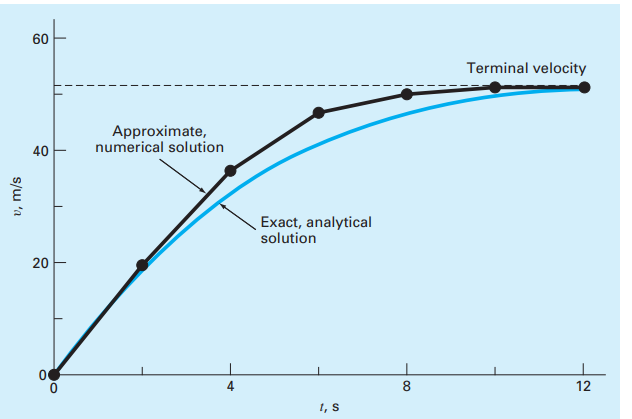
\includegraphics[width=0.75\textwidth]{fig_1.4}
			   \caption{\textsf{Comparison of the numerical and analytical solutions for the bungee jumper problem.}}
			   \label{fig_1.}
			\end{figure}


